\documentclass[12pt,a4paper]{article}
\usepackage{fontspec}
\usepackage{tgtermes}
\usepackage[top=3cm,bottom=2cm,left=3cm,right=2cm]{geometry}
\usepackage{setspace}
\usepackage{booktabs,tabularx,array}
\usepackage{enumitem}
\usepackage{float}
\usepackage{xcolor}
\usepackage{graphicx}
\usepackage{fancyhdr}
\usepackage{listings}
\usepackage{titlesec}
\usepackage[font=small,labelfont=bf,labelsep=endash]{caption}
\usepackage{tikz}
\usetikzlibrary{positioning,arrows.meta}
\usepackage[hidelinks]{hyperref}
\onehalfspacing
\sloppy\emergencystretch=3em
\renewcommand{\contentsname}{SUMÁRIO}
\renewcommand{\tablename}{Tabela}
\renewcommand{\figurename}{Figura}
\renewcommand{\refname}{REFERÊNCIAS}
\setlength{\parindent}{1.25cm}
\setlength{\parskip}{0pt}
\setlist{itemsep=2pt,topsep=4pt}
\titleformat{\section}{\normalfont\bfseries\MakeUppercase}{\thesection}{1em}{}
\titleformat{\subsection}{\normalfont\bfseries}{\thesubsection}{1em}{}
\titleformat{\subsubsection}{\normalfont\itshape\bfseries}{\thesubsubsection}{1em}{}
\titlespacing*{\section}{0pt}{18pt}{12pt}
\titlespacing*{\subsection}{0pt}{14pt}{8pt}
\newcommand{\code}[1]{\texttt{\detokenize{#1}}}
\newcolumntype{Y}{>{\raggedright\arraybackslash}X}
\definecolor{cbg}{gray}{0.95}
\lstset{basicstyle=\ttfamily\footnotesize,backgroundcolor=\color{cbg},frame=single,
  framerule=0.3pt,rulecolor=\color{gray},breaklines=true,columns=fullflexible,
  keepspaces=true,showstringspaces=false,xleftmargin=2pt,xrightmargin=2pt,
  language=Java,keywordstyle=\bfseries,commentstyle=\itshape\color{gray}}
\pagestyle{empty}

\begin{document}

% ---------- CAPA ----------
\begin{titlepage}\centering\singlespacing

\includegraphics[width=4.5cm]{../../java/img/logo.png}\\[0.8cm]
{\large UNIVERSIDADE CATÓLICA DO SALVADOR}\\[0.2cm]
{\large Evolução e Modernização de Sistemas Legados -- 2026.2}\\[2.5cm]
{\large Manuel Bahamonde Boulhosa Neto (200031998)\\
Sérgio Lopes Júnior (200026817)\\
Juvenal Rosa Alves Costa Junior (200033214)}\\[2.5cm]
{\Large\bfseries EVOLUÇÃO E MODERNIZAÇÃO DE UM SISTEMA LEGADO:\\[0.2cm]
DIAGNÓSTICO E REFATORAÇÃO DO \textit{SUPERMARKETRECEIPT REFACTORING KATA}}\\[1cm]
{\large Relatório técnico da disciplina}\vfill
{\large Salvador\\ 2026}
\end{titlepage}

% ---------- RESUMO ----------
\thispagestyle{empty}
\begin{center}\textbf{RESUMO}\end{center}
\singlespacing\noindent
Este trabalho apresenta a análise técnica, a engenharia reversa e a refatoração do \textit{SupermarketReceipt Refactoring Kata}, um sistema em Java que simula o fechamento de compra de um supermercado com promoções. O diagnóstico identificou 26 achados, entre eles um método de complexidade ciclomática 13 que concentrava todas as regras de promoção, valores monetários e quantidades representados por \code{double}, classes anêmicas, um carrinho que guardava o mesmo estado duas vezes e ausência de documentação. A equipe, dividida em três grupos, escreveu testes de caracterização antes de refatorar e aplicou, em \textit{commits} pequenos integrados por \textit{pull requests} com integração contínua, o padrão \textit{Strategy} às ofertas, os tipos \code{Money} e \code{Quantity}, a eliminação do estado duplicado e a reorganização da impressão da nota fiscal. Foram implementadas ainda duas funcionalidades novas: a oferta de pacote e o formato HTML da nota. Os testes passaram de 1 para 124, a maior complexidade ciclomática do domínio de ofertas caiu de 13 para 4 e a cobertura chegou a 100\% de linhas e de \textit{branches}. O trabalho discute as limitações do estudo, os riscos e a viabilidade de aplicar a abordagem a sistemas maiores.\par\vspace{0.5cm}
\noindent\textbf{Palavras-chave:} evolução de software; refatoração; sistemas legados; dívida técnica; testes de caracterização.
\onehalfspacing\newpage

% ---------- SUMÁRIO ----------
\thispagestyle{empty}
\tableofcontents
\newpage
\pagestyle{fancy}\fancyhf{}\fancyhead[R]{\small\thepage}\renewcommand{\headrulewidth}{0pt}

% ================= 1 INTRODUÇÃO =================
\section{Introdução}

Sistemas de software raramente são abandonados quando funcionam: eles continuam em uso e precisam receber novas regras de negócio. Quando o código acumula decisões ruins, cada mudança fica mais cara e mais arriscada. Esse processo é descrito pela literatura como evolução de software e tem na refatoração e na reengenharia as principais respostas técnicas (SOMMERVILLE, 2019; FOWLER, 2020).

Este trabalho aplica esses conceitos a um sistema real de pequeno porte, o \textit{SupermarketReceipt Refactoring Kata} (BACHE, [s.d.]). O sistema simula um caixa de supermercado: recebe os produtos de um carrinho, aplica promoções semanais e emite uma nota fiscal. Foi criado para o treino de refatoração e, por isso, reúne problemas típicos de código legado de forma concentrada, o que o torna adequado para estudar o ciclo completo de análise, diagnóstico e transformação.

\subsection{Objetivos}

O objetivo geral é diagnosticar e refatorar o sistema legado, preservando seu comportamento e melhorando sua manutenibilidade. Os objetivos específicos são:
\begin{itemize}
\item descrever o sistema e mapear suas funcionalidades e arquitetura (engenharia reversa);
\item produzir um relatório de débito técnico que quantifique acoplamento, duplicação, complexidade, documentação e manutenibilidade;
\item criar uma rede de testes de caracterização antes de alterar o código;
\item refatorar o sistema de forma incremental, com evidências de ``antes'' e ``depois'';
\item implementar funcionalidades novas sobre o código refatorado, como prova de que a evolução ficou mais barata;
\item analisar criticamente a viabilidade, os riscos e as limitações da abordagem.
\end{itemize}

\subsection{Metodologia}

O trabalho foi realizado por três integrantes, entre 10 e 23 de novembro de 2026, em um repositório público no GitHub. O código foi dividido em três grupos de classes, um por integrante: o Grupo 1 ficou com \code{Teller}, \code{Offer} e \code{SpecialOfferType}, cujo desafio era a lógica de promoções; o Grupo 2 com \code{ShoppingCart}, \code{ProductQuantity}, \code{Product} e \code{ProductUnit}, cujos desafios eram o estado duplicado do carrinho e a quantidade em \code{double}; e o Grupo 3 com \code{Receipt}, \code{ReceiptItem}, \code{Discount}, \code{ReceiptPrinter} e o catálogo, cujos desafios eram a impressão sem testes, a lista de descontos mutável e a lista longa de parâmetros.

As regras de trabalho foram: (i) escrever testes de caracterização antes de refatorar (FEATHERS, 2013); (ii) fazer cada refatoração em um \textit{commit} próprio, com os testes verdes antes e depois; (iii) integrar tudo por \textit{pull requests} com execução automática da suíte (GitHub Actions); e (iv) medir a cobertura com JaCoCo. As ferramentas foram Java 17, Maven, JUnit 5 e ApprovalTests. O estado inicial do sistema está preservado na \textit{tag} \code{legado} do repositório, que permite comparar a versão original com a refatorada.

\subsection{Organização do relatório}

A seção 2 apresenta a fundamentação teórica. A seção 3 descreve o sistema, o diagnóstico, a refatoração aplicada, as funcionalidades novas, os resultados e a colaboração da equipe. A seção 4 traz a análise crítica e de viabilidade. A seção 5 conclui o trabalho.

% ================= 2 FUNDAMENTAÇÃO =================
\section{Fundamentação teórica}

\subsection{Sistemas legados e evolução de software}

Um sistema legado costuma ser definido por características como tecnologia obsoleta, importância vital para a organização e ausência de documentação. Em um mapeamento da literatura entre 1995 e 2015, Martins, Chervenski e Bordin (2017) observam que essas são as características mais frequentes nas definições publicadas. O sistema estudado neste trabalho foge do primeiro critério (usa Java 17 e ferramentas atuais), mas apresenta o terceiro (nenhuma documentação) e, principalmente, problemas de projeto que dificultam a mudança. É, portanto, um legado por projeto e não por tecnologia, o que reforça que a dificuldade de evoluir um sistema não depende só da idade das ferramentas.

Lehman (1980) formulou leis da evolução de software. Duas delas são especialmente relevantes aqui: um sistema em uso precisa ser continuamente adaptado, sob pena de se tornar cada vez menos útil, e sua complexidade cresce a menos que haja trabalho deliberado para reduzi-la. Sommerville (2019) trata a evolução como parte do ciclo de vida e distingue manutenção corretiva, adaptativa e perfectiva, além da reengenharia, que reestrutura o sistema sem mudar suas funções.

\subsection{Dívida técnica}

A metáfora da dívida técnica foi proposta por Cunningham (1992): decisões rápidas ou inadequadas permitem avançar hoje, mas geram ``juros'', na forma de esforço extra em todas as mudanças futuras, até que a dívida seja paga por meio de refatoração. Neste trabalho, o relatório de débito técnico organiza os problemas encontrados em cinco dimensões: acoplamento, duplicação, complexidade ciclomática, falta de documentação e manutenibilidade.

\subsection{\textit{Code smells} e refatoração}

Refatoração é a alteração da estrutura interna do código sem mudar seu comportamento observável. Fowler (2020) cataloga \textit{code smells}, como função longa, obsessão por primitivos, classes de dados e nomes misteriosos, e as refatorações que os tratam, como \textit{Extract Function}, \textit{Replace Conditional with Polymorphism} e \textit{Replace Primitive with Object}. Martin (2011) complementa com princípios de legibilidade: nomes expressivos, funções pequenas e ausência de duplicação.

\subsection{Testes de caracterização}

Antes de alterar código sem testes, é preciso registrar o que ele faz hoje. Feathers (2013) chama de testes de caracterização aqueles que descrevem o comportamento atual, inclusive os defeitos, para que uma refatoração possa ser verificada: se o teste continua passando, o comportamento foi preservado. Uma consequência prática, observada neste trabalho, é que uma suíte verde só protege o que ela cobre.

\subsection{Métricas}

A complexidade ciclomática (MCCABE, 1976) mede o número de caminhos independentes de um método e, na prática, é obtida contando os pontos de decisão e somando um. Valores acima de 10 são comumente tratados como sinal de que o método deve ser dividido. A cobertura de testes mede a proporção de linhas e de \textit{branches} executados pela suíte; ela indica o que não é testado, mas não garante a qualidade dos testes.

\subsection{Padrão \textit{Strategy}}

O padrão \textit{Strategy} (GAMMA \textit{et al}., 2000) encapsula uma família de algoritmos em classes intercambiáveis atrás de uma interface comum. Ele é a forma clássica de substituir uma cadeia condicional que escolhe um comportamento por tipo, e é a base da refatoração das promoções descrita adiante.

% ================= 3 DESENVOLVIMENTO =================
\section{Desenvolvimento}

\subsection{O sistema legado}

O \textit{SupermarketReceipt Refactoring Kata}, na versão Java, tem cerca de 200 linhas de produção em 11 classes de um único pacote, mais uma classe de impressão que estava na pasta de testes. O sistema não possui interface nem ponto de entrada: suas funcionalidades são exercitadas por testes. A Tabela~\ref{tab:func} resume o que ele faz.

\begin{table}[H]\centering\small\singlespacing
\begin{tabularx}{\textwidth}{>{\raggedright\arraybackslash}p{4.4cm}Y}
\toprule \textbf{Funcionalidade} & \textbf{Descrição} \\ \midrule
Catálogo e produtos & Preço unitário por produto; produto vendido por unidade ou por peso (quilo). \\
Carrinho de compras & Adição de produtos com quantidade; acúmulo da quantidade por produto. \\
Ofertas especiais & Quatro tipos por produto: 10\% de desconto, leve 3 e pague 2, 2 por valor fixo e 5 por valor fixo. \\
Fechamento da compra & Geração da nota com uma linha por item e aplicação das ofertas. \\
Nota fiscal e impressão & Itens, descontos negativos e total; texto em colunas. \\
\bottomrule\end{tabularx}
\caption{Funcionalidades do sistema legado.}\label{tab:func}\end{table}

\begin{figure}[H]\centering
\includegraphics[width=\textwidth]{../../java/supermarket.png}
\caption{Diagrama de classes do sistema legado, gerado pelo grupo na etapa de engenharia reversa.}\label{fig:uml}
\end{figure}

Do ponto de vista lógico, identificaram-se cinco componentes: dados de domínio (\textit{records} e \textit{enums} sem comportamento), o contrato de catálogo, a orquestração (\code{Teller}), as regras de promoção (todas dentro de \code{ShoppingCart.handleOffers}) e a nota fiscal com sua impressão. O \code{ShoppingCart} é o ponto de acoplamento: dependia de sete tipos e era a única classe com regra de negócio.

\subsection{Diagnóstico técnico}

\subsubsection{Método}

A engenharia reversa seguiu um roteiro de cinco passos: preparação (clonar, executar os testes e levantar os arquivos), leitura panorâmica das classes, localização do ponto de entrada (os testes, já que não há \code{main}), leitura guiada do único cenário existente e leitura aprofundada de cada classe e método. Os achados foram classificados pelo catálogo de Fowler (2020). Complementaram a análise o diagrama de classes (Figura~\ref{fig:uml}) e cartões CRC de todas as classes. Por se tratar de um sistema pequeno, as métricas foram obtidas por contagem manual, em vez de ferramentas como SonarQube, cujo ganho seria pequeno para cerca de 280 linhas.

\subsubsection{Relatório de débito técnico}

Foram registrados 26 achados (L-01 a L-26). A Tabela~\ref{tab:debito} os consolida nas cinco dimensões.

\begin{table}[H]\centering\small\singlespacing
\begin{tabularx}{\textwidth}{>{\raggedright\arraybackslash}p{3.2cm}Y}
\toprule \textbf{Dimensão} & \textbf{Diagnóstico} \\ \midrule
Acoplamento & \code{ShoppingCart} dependia de 7 tipos e alterava a nota fiscal diretamente (\textit{Feature Envy}); o \code{Teller} guardava as ofertas e as repassava ao carrinho a cada fechamento. \\
Duplicação & O mesmo tipo de oferta era testado em mais de um \code{if}; a fórmula de desconto se repetia em quatro blocos; as constantes 2, 3 e 5 apareciam como variável e como literais. \\
Complexidade & \code{handleOffers} com complexidade ciclomática 13 (12 decisões); os demais métodos, entre 1 e 3. \\
Documentação & Nenhum Javadoc; nomes pouco expressivos (\code{x}, \code{numberOfXs}, \code{quantityAsInt}); nenhum documento de arquitetura. \\
Manutenibilidade & Dinheiro e quantidade em \code{double}; classes anêmicas; coleção mutável exposta; classe de impressão fora do código de produção; um único pacote; adicionar uma oferta exigia editar o método mais complexo. \\
\bottomrule\end{tabularx}
\caption{Débito técnico do sistema legado por dimensão.}\label{tab:debito}\end{table}

Os achados foram priorizados em três faixas. Alta prioridade: a cadeia condicional de ofertas (achados L-04, L-07, L-19, L-20 e L-21) e o dinheiro em \code{double}. Média: classes anêmicas, nomes confusos, encapsulamento e estrutura de pacotes. Baixa: documentação e limpeza do repositório.

\subsection{Estratégia de refatoração}

O sistema tinha um único teste efetivo. Antes de refatorar, foram escritos testes de caracterização para todos os tipos de oferta (abaixo do mínimo, com múltiplos do grupo, por peso, com quantidades somadas em linhas separadas), para o carrinho, para a nota e para a impressão, inclusive registrando defeitos do legado. Com 37 testes, mediu-se a cobertura de linha de base: 98,9\% das linhas (88 de 89) e 100\% dos \textit{branches} (28 de 28). A partir daí, cada refatoração foi feita em um \textit{commit} próprio, e cada \textit{pull request} só era integrado com a suíte verde no CI. A \textit{branch} principal tem regra de proteção que exige esse fluxo.

\subsection{Refatoração aplicada}

\subsubsection{Grupo 1: ofertas e caixa}

O método \code{ShoppingCart.handleOffers} concentrava todas as regras de promoção em uma cadeia de \code{if}. Ele foi substituído por uma interface \code{OfferStrategy} e três implementações (\code{PercentDiscountOffer}, \code{ThreeForTwoOffer} e \code{QuantityForAmountOffer}, esta última atendendo às ofertas de 2 e de 5 por valor fixo). O cadastro das ofertas saiu do \code{Teller} para a classe \code{SpecialOffers}, e o record anêmico \code{Offer} foi removido. A Figura~\ref{fig:arq} mostra a arquitetura resultante.

\begin{figure}[H]\centering
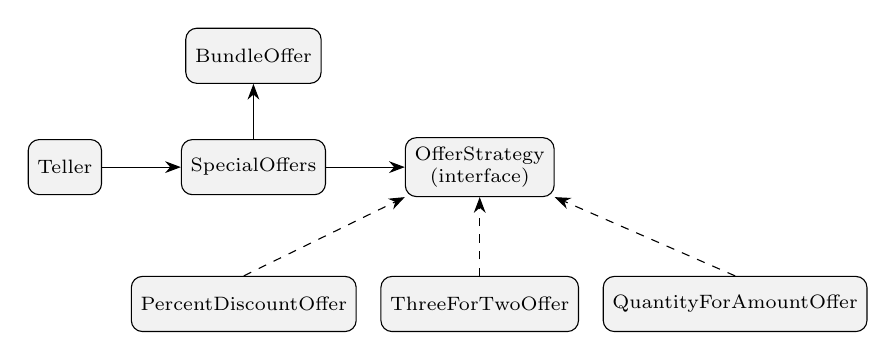
\begin{tikzpicture}[box/.style={draw,rounded corners,align=center,minimum height=7mm,font=\scriptsize,fill=cbg},>={Stealth[length=2mm]},node distance=9mm]
\node[box] (teller) {Teller};
\node[box,right=10mm of teller] (so) {SpecialOffers};
\node[box,right=10mm of so] (os) {OfferStrategy\\(interface)};
\node[box,above=7mm of so] (bundle) {BundleOffer};
\node[box,below=10mm of os] (t2) {ThreeForTwoOffer};
\node[box,left=3mm of t2] (t1) {PercentDiscountOffer};
\node[box,right=3mm of t2] (t3) {QuantityForAmountOffer};
\draw[->] (teller) -- (so);
\draw[->] (so) -- (os);
\draw[->] (so) -- (bundle);
\draw[->,dashed] (t1.north) -- (os.south west);
\draw[->,dashed] (t2.north) -- (os.south);
\draw[->,dashed] (t3.north) -- (os.south east);
\end{tikzpicture}
\caption{Arquitetura das ofertas após a refatoração (setas tracejadas indicam implementação).}\label{fig:arq}
\end{figure}

\noindent O trecho abaixo mostra o ``antes'' da regra do leve 3 e pague 2, no meio da cadeia condicional, e o ``depois'', em sua própria classe.

\begin{lstlisting}
// ANTES (ShoppingCart.handleOffers, trecho)
int x = 1;
if (offer.offerType() == SpecialOfferType.THREE_FOR_TWO) {
    x = 3;
} else if (offer.offerType() == SpecialOfferType.TWO_FOR_AMOUNT) {
    x = 2;
    if (quantityAsInt >= 2) { /* ... */ }
} if (offer.offerType() == SpecialOfferType.FIVE_FOR_AMOUNT) {
    x = 5;
}
int numberOfXs = quantityAsInt / x;
if (offer.offerType() == SpecialOfferType.THREE_FOR_TWO && quantityAsInt > 2) {
    double discountAmount = quantity * unitPrice
        - ((numberOfXs * 2 * unitPrice) + quantityAsInt % 3 * unitPrice);
    discount = new Discount(p, "3 for 2", -discountAmount);
}
\end{lstlisting}
\begin{lstlisting}
// DEPOIS (ThreeForTwoOffer)
public Optional<Discount> discountFor(Product product, Quantity quantity, Money unitPrice) {
    int units = quantity.wholeUnits();
    if (units < GROUP_SIZE) {
        return Optional.empty();
    }
    int completeGroups = units / GROUP_SIZE;
    Money fullPrice = unitPrice.times(quantity);
    Money payable = unitPrice.times(completeGroups * PAID_PER_GROUP + units % GROUP_SIZE);
    return Optional.of(new Discount(product, "3 for 2", payable.minus(fullPrice)));
}
\end{lstlisting}

A prova de que a extensão ficou mais barata está em um teste: uma oferta nova pode ser criada com uma expressão \textit{lambda}, sem alterar nenhuma classe existente.

\subsubsection{Grupo 2: carrinho e quantidades}

O carrinho guardava a mesma informação em duas estruturas, a lista de itens adicionados e um mapa com as quantidades agregadas, ambas atualizadas em \code{addItemQuantity}. A refatoração \textit{Replace Derived Variable with Query} eliminou o mapa: as quantidades por produto passam a ser calculadas sob demanda a partir da lista. Os construtores de \code{Product} e \code{ProductQuantity} passaram a validar seus dados, e a regra de que unidades discretas só aceitam quantidades inteiras foi movida para \code{ProductUnit}.

\begin{lstlisting}
// ANTES
private final List<ProductQuantity> items = new ArrayList<>();
private final Map<Product, Double> productQuantities = new HashMap<>();

public void addItemQuantity(Product product, double quantity) {
    items.add(new ProductQuantity(product, quantity));
    if (productQuantities.containsKey(product)) {
        productQuantities.put(product, productQuantities.get(product) + quantity);
    } else {
        productQuantities.put(product, quantity);
    }
}
\end{lstlisting}
\begin{lstlisting}
// DEPOIS
private final List<ProductQuantity> items = new ArrayList<>();

Map<Product, Quantity> productQuantities() {
    Map<Product, Quantity> quantities = new HashMap<>();
    for (ProductQuantity item : items) {
        quantities.merge(item.product(), item.quantity(), Quantity::plus);
    }
    return Collections.unmodifiableMap(quantities);
}
\end{lstlisting}

\subsubsection{Grupo 3: nota fiscal e impressão}

A classe \code{ReceiptPrinter}, que era código de produção dentro da pasta de testes, foi movida para o pacote principal e coberta por testes antes de ser alterada. Seguiram-se refatorações pequenas: constantes no lugar de literais, \textit{Decompose Conditional} na condição da linha de quantidade, a regra de formato por unidade movida para o dado e o total do item calculado em vez de armazenado, o que reduziu \code{Receipt.addProduct} de quatro para três parâmetros. A lista de descontos passou a ser devolvida de forma imutável, como já era a lista de itens, e uma interface \code{ReceiptPrinterFormatter} permitiu acrescentar novos formatos.

\begin{lstlisting}
// ANTES
if (item.quantity() != 1) {
    line += "  " + presentPrice(item.price()) + " * " + presentQuantity(item) + "\n";
}
// DEPOIS
if (!item.hasSingleQuantity()) {
    line.append("  " + ReceiptFormat.price(item.price()) + " * " + ReceiptFormat.quantity(item) + "\n");
}
\end{lstlisting}

\subsubsection{Refatorações transversais: \code{Money} e \code{Quantity}}

Dois tipos de valor atravessaram as classes dos três grupos. O tipo \code{Money}, baseado em \code{BigDecimal} com duas casas e arredondamento \textit{half-up}, substituiu o \code{double} em todos os valores monetários (catálogo, ofertas, descontos, itens e total). O tipo \code{Quantity}, decimal exato com três casas, substituiu o \code{double} das quantidades e concentrou em um único método, \code{wholeUnits()}, o \textit{cast} para \code{int} que estava espalhado pelas regras de oferta. As duas mudanças aplicam \textit{Replace Primitive with Object} (FOWLER, 2020). Um ganho verificável é a soma exata de quilos: 0,1 kg mais 0,2 kg resulta exatamente em 0,300 kg, e não em 0,30000000000000004.

\subsection{Funcionalidades novas sobre o código refatorado}

\textbf{Oferta de pacote.} O enunciado do \textit{kata} pede um desconto de 10\% quando o cliente leva todos os itens de um conjunto, descontando apenas pacotes completos. A classe \code{BundleOffer} implementa a regra: com uma escova de dentes (R\$\,0,99) e uma pasta de dente (R\$\,1,79), o desconto é de 10\% de R\$\,2,78, ou seja R\$\,0,28 após o arredondamento, e o total é R\$\,2,50. Com duas escovas e uma pasta há um único pacote completo, e o desconto é o mesmo. Por envolver vários produtos, ela é um tipo separado de \code{OfferStrategy}, e seu desconto soma-se às ofertas por produto. Foram escritos testes para os cenários do enunciado e para os casos-limite.

\textbf{Formato HTML da nota.} A classe \code{ReceiptPrinterHtml} gera a nota como tabela HTML (itens, linha de quantidade, descontos e total), escapando os textos, e reaproveita o formato de preços e quantidades da impressão em texto.

\subsection{Resultados}

A Tabela~\ref{tab:result} compara o sistema legado com a versão final. As métricas de complexidade foram contadas manualmente e a cobertura foi medida com JaCoCo.

\begin{table}[H]\centering\small\singlespacing
\begin{tabularx}{\textwidth}{>{\raggedright\arraybackslash}p{5.3cm}>{\raggedright\arraybackslash}p{3.7cm}Y}
\toprule \textbf{Indicador} & \textbf{Legado} & \textbf{Final} \\ \midrule
Testes automatizados & 1 (na \textit{tag} \code{legado}) & 124, todos passando \\
Cobertura de linhas e de \textit{branches} & 98,9\% e 100\% (medida com 37 testes, antes de refatorar) & 100\% e 100\% (243 de 243 linhas; 66 de 66 \textit{branches}) \\
Maior complexidade ciclomática no domínio de ofertas & 13 (\code{handleOffers}) & 4 (\code{OfferStrategies.from}) \\
Estruturas que guardam o conteúdo do carrinho & 2 (lista e mapa) & 1 (lista) \\
Valores monetários & \code{double} & \code{Money} \\
Quantidades & \code{double} e \textit{cast} para \code{int} & \code{Quantity} \\
Classes de produção com Javadoc & 0 & 10 de 23 \\
Dependências de \code{ShoppingCart} & 7 tipos & 3 tipos \\
Dependências de \code{Teller} & 7 tipos & 12 tipos (piorou) \\
Funcionalidades novas & -- & 2 (pacote e HTML) \\
\bottomrule\end{tabularx}
\caption{Comparação entre o legado e a versão final.}\label{tab:result}\end{table}

Um resultado negativo merece registro: as dependências do \code{Teller} aumentaram de 7 para 12 tipos, porque ele passou a delegar por \code{SpecialOffers}, \code{OfferStrategies} e \code{OfferStrategy} e a usar \code{BundleOffer}, \code{Money} e \code{Quantity}. A responsabilidade da classe diminuiu, mas a contagem de tipos que ela conhece cresceu. Reduzir esse número exigiria dividir o código em pacotes, o que ficou como trabalho futuro.

\subsection{Mudanças de comportamento e lições}

Nem toda alteração foi uma refatoração pura, e as diferenças foram registradas nos testes e na documentação do projeto:
\begin{itemize}
\item \textbf{Arredondamento ao centavo.} Com \code{Money}, descontos e totais são arredondados: 10\% de uma escova de R\$\,0,99 passou de 0,099 para R\$\,0,10, e as descrições mostram duas casas (``2 for 1.50'' em vez de ``2 for 1.5'').
\item \textbf{Total do item derivado.} Ao calcular o total do item em vez de armazená-lo, três testes de impressão mudaram de valor esperado, porque os testes antigos informavam totais incoerentes com a quantidade e o preço.
\item \textbf{Validação na criação.} Objetos inválidos (nome vazio, quantidade negativa ou fracionária para produto por unidade) agora falham com \code{IllegalArgumentException}.
\end{itemize}

Houve também um defeito introduzido durante a refatoração e corrigido na revisão. Ao extrair a condição da linha de quantidade, a expressão \code{item.quantity() != 1} foi trocada por \code{item.quantity() > 1}, e quantidades menores que 1 (por exemplo, 0,5 kg) deixaram de imprimir a linha de quantidade. A suíte permaneceu verde porque nenhum teste usava quantidade abaixo de 1. O teste que reproduz o defeito foi escrito, e a condição original foi restaurada. O episódio ilustra a lição de Feathers (2013): uma suíte verde só protege o que ela cobre, e os casos-limite precisam ser testados antes de alterar uma condição.

\subsection{Planos de atualização e de modularização}

Cada grupo elaborou dois planos. O plano de atualização tecnológica define fases (medição de cobertura, análise estática, \textit{Maven Wrapper}, recursos do Java 17, eventual migração para o Java 21, tipos \code{Money} e \code{Quantity}, Javadoc) e estratégias de evolução: ofertas extensíveis, oferta de pacote, cadastro de ofertas separado do caixa, carga das ofertas semanais por arquivo de configuração com período de validade e, mais adiante, exposição por uma API. Como o sistema tem cerca de 280 linhas, a quebra em microsserviços não se justifica; recomenda-se um monólito modular. O plano de modularização descreve a arquitetura-alvo, a sequência de refatorações e as metas. Nele, a divisão em pacotes (\code{offer}, \code{checkout}) foi adiada por criar dependência circular enquanto \code{Teller} e \code{ShoppingCart} compartilham o pacote das estratégias.

\subsection{Colaboração da equipe}

O histórico do GitHub registra a participação dos integrantes. Entre 10 e 23 de novembro foram integrados 36 \textit{pull requests}, todos com execução da suíte no CI, e a Tabela~\ref{tab:contrib} mostra a distribuição.

\begin{table}[H]\centering\small\singlespacing
\begin{tabularx}{\textwidth}{>{\raggedright\arraybackslash}p{6cm}>{\centering\arraybackslash}p{3cm}Y}
\toprule \textbf{Integrante} & \textbf{\textit{Commits}} & \textbf{\textit{Pull requests} integrados} \\ \midrule
Sérgio Lopes Júnior & 60 & 18 \\
Manuel Bahamonde Boulhosa Neto & 42 & 16 \\
Juvenal Rosa Alves Costa Junior & 4 & 2 \\
\bottomrule\end{tabularx}
\caption{Contribuições no repositório (\textit{commits} sem \textit{merges}, a partir de 10/11/2026).}\label{tab:contrib}\end{table}

A distribuição é desigual. Além dos números, o Grupo 2 teve seu desafio de quantidade concluído com o tipo \code{Quantity}, implementado em acordo com a equipe e integrado por \textit{pull request}, e as alterações transversais (\code{Money}, \code{Quantity}) exigiram atualizar arquivos dos três grupos.

% ================= 4 ANÁLISE CRÍTICA =================
\section{Análise crítica e viabilidade}

\subsection{Visão de negócio}

No cenário do sistema, as promoções mudam toda semana. Antes da refatoração, criar um tipo de oferta exigia editar o método mais complexo do sistema (complexidade 13) e o \textit{enum}, com risco de afetar as ofertas existentes. Depois, uma oferta nova é uma classe ou uma \textit{lambda}, testada de forma isolada, o que reduz o custo e o risco de cada mudança semanal. O tipo \code{Money} elimina diferenças de arredondamento entre o que a nota mostra e o que ela soma, o que importa para a confiança do cliente e para a conciliação do caixa. A oferta de pacote, pedida pelo próprio dono do sistema no enunciado, foi implementada em poucos \textit{commits} sobre o código refatorado, o que serve de evidência prática do ganho.

\subsection{Prazo e esforço}

O trabalho foi concluído em 14 dias corridos por três pessoas, em um sistema de cerca de 280 linhas. Esse resultado não deve ser extrapolado de forma linear: em um sistema real, com banco de dados, interface e muito mais código, o custo da escrita de testes de caracterização e da coordenação entre equipes cresce de forma desproporcional. A parte de maior retorno foi a rede de testes feita primeiro, que permitiu refatorar com segurança.

\subsection{Riscos}

\begin{table}[H]\centering\small\singlespacing
\begin{tabularx}{\textwidth}{>{\raggedright\arraybackslash}p{4.4cm}>{\raggedright\arraybackslash}p{2cm}Y}
\toprule \textbf{Risco} & \textbf{Impacto} & \textbf{Tratamento e resultado} \\ \midrule
Regressão de comportamento & Alto & Testes de caracterização e CI em todo \textit{pull request}; houve um defeito introduzido e detectado na revisão (seção 3.7). \\
Conflitos entre grupos & Médio & \textit{Pull requests} pequenos e avisos; as mudanças de \code{Money} e \code{Quantity} atravessaram arquivos dos três grupos e foram feitas de forma atômica, com os testes atualizados. \\
Mudança de comportamento não percebida & Médio & Arredondamento e validações registrados em testes e na documentação. \\
Participação desigual na equipe & Médio & Visível no histórico do GitHub (Tabela~\ref{tab:contrib}); exige acompanhamento. \\
Métricas manuais sujeitas a erro & Baixo & Contagens conferidas por revisão; a cobertura vem de ferramenta. \\
\bottomrule\end{tabularx}
\caption{Riscos do projeto e seu tratamento.}\end{table}

\subsection{Limitações}

Há limitações que devem ser reconhecidas. Primeiro, o \textit{kata} é pequeno e foi criado para treino, e por isso não representa os desafios de um legado real, como dados persistidos, concorrência, integrações e falta de especificação; as conclusões valem sobretudo para a técnica, não para a escala. Segundo, a complexidade foi contada manualmente e se refere ao domínio de ofertas, não a uma medição automática do sistema inteiro. Terceiro, a cobertura de 100\% não garante qualidade: o defeito descrito na seção 3.7 passou por uma suíte verde. Quarto, ficaram pendentes a decisão sobre unificar \code{Product} e \code{ProductQuantity} (achado L-13), a divisão em pacotes, a análise estática automatizada e a evolução do campo de valor das ofertas, que ainda recebe \code{double} na API pública do \code{Teller}.

\subsection{Trabalho futuro}

Os próximos passos recomendados são dividir o código em pacotes por responsabilidade, adotar análise estática no CI, manter as ofertas semanais em arquivo de configuração com período de validade, acrescentar o desconto de pacote ao cadastro externo e, se houver demanda, expor o cálculo de nota por uma API.

% ================= 5 CONCLUSÃO =================
\section{Conclusão}

O trabalho percorreu o ciclo completo de evolução de um sistema legado: descrição, engenharia reversa, diagnóstico de débito técnico, rede de testes, refatoração incremental e evolução por novas funcionalidades. A principal conclusão é que a ordem importa: foi a escrita de testes de caracterização antes de qualquer alteração que tornou seguras as mudanças maiores, como a troca da cadeia condicional por \textit{Strategy} e a troca de \code{double} por \code{Money} e \code{Quantity}.

Os resultados medidos sustentam o ganho: os testes passaram de 1 para 124, a complexidade do maior método do domínio de ofertas caiu de 13 para 4, o carrinho deixou de guardar estado duplicado, valores monetários e quantidades ganharam tipos próprios e duas funcionalidades novas foram implementadas sobre o código refatorado, uma delas com uma regra que envolve vários produtos. Também houve resultados negativos e lições, como o aumento das dependências do \code{Teller}, o defeito introduzido e corrigido durante a refatoração, as mudanças de comportamento do arredondamento e a participação desigual da equipe, todos registrados de forma transparente.

Fica como aprendizado que refatorar não é reescrever: cada passo foi pequeno, verificável e integrado por \textit{pull request}, e o repositório mantém a versão original marcada para comparação. Os próximos passos, descritos nos planos de cada grupo, concentram-se em pacotes, análise estática e configuração externa das ofertas.

% ================= REFERÊNCIAS =================
\newpage
\section*{REFERÊNCIAS}
\addcontentsline{toc}{section}{REFERÊNCIAS}
\begin{singlespace}\raggedright\noindent
BACHE, Emily. \textbf{SupermarketReceipt-Refactoring-Kata}. [\textit{S. l.}]: GitHub, [s.d.]. Disponível em: https://github.com/emilybache/SupermarketReceipt-Refactoring-Kata. Acesso em: 23 nov. 2026.

\vspace{12pt}\noindent CUNNINGHAM, Ward. The WyCash portfolio management system. In: OOPSLA '92 EXPERIENCE REPORT, 1992, Vancouver. \textbf{Anais} [...]. [\textit{S. l.}]: ACM, 1992.

\vspace{12pt}\noindent FEATHERS, Michael. \textbf{Trabalho eficaz com código legado}. Porto Alegre: Bookman, 2013.

\vspace{12pt}\noindent FOWLER, Martin. \textbf{Refatoração}: aperfeiçoando o design de código existente. 2. ed. São Paulo: Novatec, 2020.

\vspace{12pt}\noindent GAMMA, Erich \textit{et al}. \textbf{Padrões de projeto}: soluções reutilizáveis de software orientado a objetos. Porto Alegre: Bookman, 2000.

\vspace{12pt}\noindent LEHMAN, Meir M. Programs, life cycles, and laws of software evolution. \textbf{Proceedings of the IEEE}, [\textit{s. l.}], v. 68, n. 9, p. 1060-1076, set. 1980.

\vspace{12pt}\noindent MARTIN, Robert C. \textbf{Código limpo}: habilidades práticas do Agile software. Rio de Janeiro: Alta Books, 2011.

\vspace{12pt}\noindent MARTINS, Daniele; CHERVENSKI, Alex; BORDIN, Andréa. Identificação de características de sistemas legados a partir da análise de conteúdo da literatura. In: ESCOLA REGIONAL DE ENGENHARIA DE SOFTWARE, 1., 2017, Alegrete. \textbf{Anais} [...]. Porto Alegre: SBC, 2017. p. 81-88. Disponível em: https://sol.sbc.org.br/index.php/eres/article/view/10084. Acesso em: 23 nov. 2026.

\vspace{12pt}\noindent MCCABE, Thomas J. A complexity measure. \textbf{IEEE Transactions on Software Engineering}, [\textit{s. l.}], v. SE-2, n. 4, p. 308-320, dez. 1976.

\vspace{12pt}\noindent SOMMERVILLE, Ian. \textbf{Engenharia de software}. 10. ed. São Paulo: Pearson Education do Brasil, 2019.
\end{singlespace}
\end{document}
